% =====================================================================================================
\section{Security Evaluation}\label{sec:security}
\textit{Setup.} We measure what a keyless observer can reconstruct. For every frame we take the better of two pictures: the protected stream decoded as is, and a \emph{replacement attack} that substitutes fixed guesses for the encrypted values and re-encodes a valid JPEG. Leakage is the edge correlation $\rho_E$, the Pearson correlation between the Sobel gradient magnitudes of this picture and of the original ($\rho_E = 0$: no outline); it is insensitive to brightness and contrast, which a learned attacker recovers from global statistics. We also report SSIM~\cite{ssim}. Sources are a synthetic scene, \NumClips{} private clips that we analyse but do not reproduce, \NumOpenClips{} openly licensed films of the Blender Foundation and the 24 Kodak images, at 320$\times$240. The protected streams of \AllDecode{} six levels decode without error in \Decoders, as Lemma~\ref{lem:format} requires.

\subsection{Outline leakage}\label{sec:leakage}
\begin{figure*}[t]
\centering
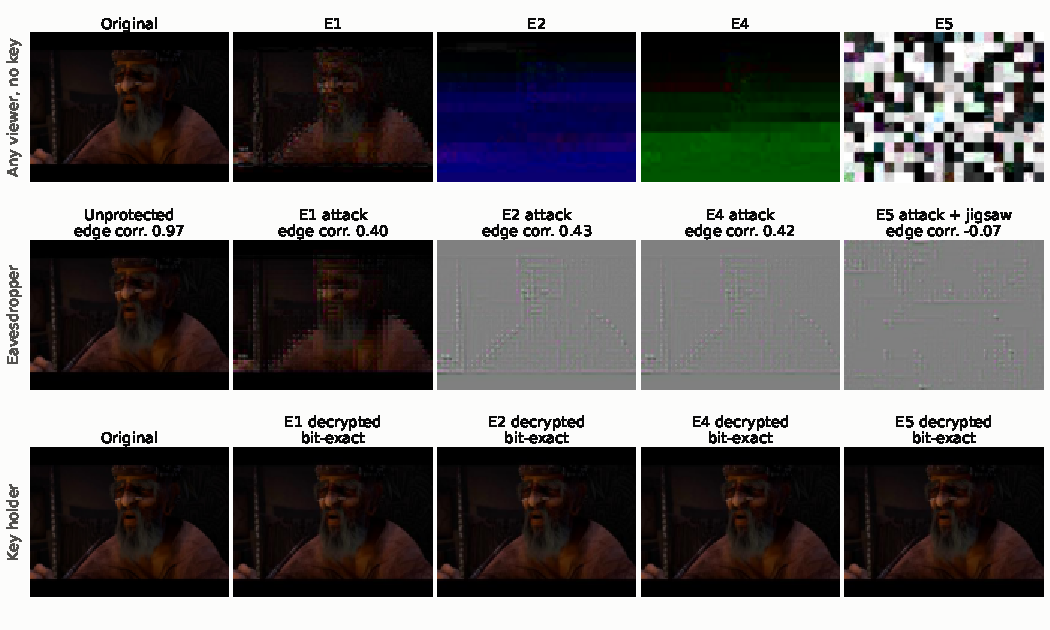
\includegraphics[width=0.62\textwidth]{figures/fig_visual_grid.pdf}
\caption{One frame of the Sintel trailer (\copyright{} Blender Foundation, CC~BY~3.0) per protection level. Top: what any viewer shows without the key. Middle: the eavesdropper's best reconstruction (for E5 after the jigsaw solver) with its edge correlation. Bottom: the key holder's output, bit-exact.}
\label{fig:grid}
\end{figure*}
% generated by paper/make_assets.py from paper/data -- do not edit
\begin{table}[t]
\caption{Outline leakage: edge correlation between the original and the eavesdropper's best keyless reconstruction (decode or replacement attack; 0 = no outline), up to 20 frames per source; frames without edges are skipped. The first row is the fraction of payload bits encrypted.}
\label{tab:leakage}
\centering\small\setlength{\tabcolsep}{4pt}
\resizebox{\columnwidth}{!}{%
\begin{tabular}{lrrrrrr}
\toprule
Source & E0 & E1 & E2 & E3 & E4 & E5 \\
\midrule
Enc.\ share & 0.00 & 0.11 & 0.13 & 0.26 & 0.30 & 0.31 \\
\midrule
Synthetic & 1.00 & 0.38 & 0.36 & 0.37 & 0.37 & 0.00 \\
Trailer A & 0.99 & 0.47 & 0.34 & 0.34 & 0.33 & 0.01 \\
Trailer B & 0.99 & 0.58 & 0.27 & 0.31 & 0.30 & 0.02 \\
Talk A & 0.99 & 0.50 & 0.44 & 0.44 & 0.44 & -0.00 \\
Talk B & 0.99 & 0.49 & 0.38 & 0.44 & 0.43 & 0.01 \\
Sintel & 0.99 & 0.35 & 0.25 & 0.26 & 0.27 & -0.00 \\
Tears of Steel & 0.99 & 0.47 & 0.34 & 0.35 & 0.43 & -0.01 \\
Kodak & 0.99 & 0.39 & 0.32 & 0.33 & 0.30 & 0.00 \\
\bottomrule
\end{tabular}}
\end{table}

Under E1--E4 the eavesdropper sees the outline of the scene (edge correlation \LeakEOneFourMin--\LeakEOneFourMax, Table~\ref{tab:leakage}, Fig.~\ref{fig:grid}), and encrypting amplitudes in addition to signs does not reduce it, because positions and size categories stay public. E5 removes the outline (\LeakEFiveMin{} to \LeakEFiveMax) for \CostEfive\,\% encrypted bits, against \CostEfour\,\% for E4, at \RiOverheadOneMin--\RiOverheadOneMax\,\% more bytes for the restart markers. Longer restart intervals would cost less, but a beam-search solver that chains segments by border continuity links many of them to their true successor at 32 MCUs per segment, so we keep one MCU per segment.

\subsection{Published schemes under the same attacks}\label{sec:bench}
\begin{figure}[t]
\centering
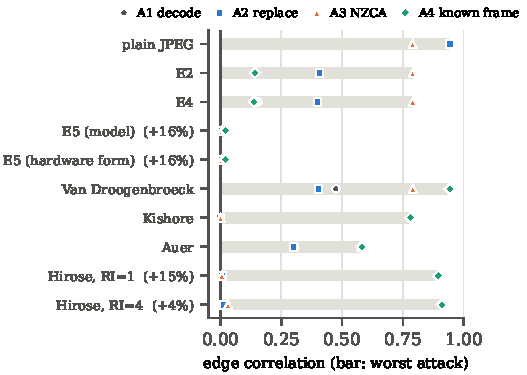
\includegraphics[width=\columnwidth]{figures/fig_bench.pdf}
\caption{SVE-Bench: edge correlation of every scheme under each attack, pooled over \BenchSources{} sources; the bar ends at the worst attack. Byte cost over plain JPEG in brackets when above 2\,\%.}
\label{fig:bench}
\end{figure}
Leakage numbers from different papers are not comparable, so we re-implemented four format-compliant schemes~\cite{vandroogenbroeck2002,kishore2015,auer2013,hirose2024} with our keystream and scored them and ours under the same four attacks on \BenchFrames{} frames of \BenchSources{} sources (Fig.~\ref{fig:bench}): A1 decoding, A2 replacement, A3 non-zero counting (a picture built from the number of non-zero coefficients per block~\cite{hirose2024}), and A4, a known-plaintext attacker that recovers the permutation and keystream bits of one frame and applies them to the next. At its strongest attack every published scheme leaks \BenchPubMin--\BenchPubMax. Fixed key material falls to A4, among them Hirose et al.\ with a restart marker after every block (\BenchHiroseOneCross), although it costs about as many bytes as E5. E1--E4 sit at the non-zero-counting ceiling of plain JPEG (\BenchPlainNzca). E5, keyed anew per frame (Proposition~\ref{prop:perm}), stays at or below \BenchEfiveMax{} in both its model and hardware form; the mechanism is the one of Hirose et al., the difference is the per-frame key.

\subsection{Stronger attackers}
\textit{Puzzle solvers and chosen plaintext.} A greedy solver in the style of~\cite{pomeranz2011} and a minimum-spanning-tree solver with gradient compatibility~\cite{gallagher2012}, both of which reassemble unencrypted shuffled tiles well, place at most \JigsawNeighboursMax{} and \MstNbMax\,\% of E5 neighbours correctly, i.e.\ chance: the signs and amplitudes are also encrypted, so tile borders no longer match. A chosen-plaintext attacker who films a pattern that reveals one frame's permutation~\cite{li2025shuffle} places \CpaPlacedEfive\,\% of the next frame's tiles, because the permutation comes from the frame nonce.

\textit{Sign recovery.} The linear program of Lin et al.~\cite{lin2024} recovers \SrLinSignsMin--\SrLinSignsMax\,\% of the signs in its own setting, where only a few signs per block are unknown, but \SrEoneSigns\,\% of E1's and \SrEtwoSigns\,\% of E2's (chance 50\,\%) on \SrFrames{} frames of \SrSources{} source sets.

\textit{Learned attackers.} A U-Net~\cite{unet} trained on \LearnBigTrain{} frames and tested on unseen sources breaks E1 (edge correlation \LearnEoneEdge, SSIM \LearnEoneSsim; replacement attack \ReplEoneEdge), adds little to the outline under E2 and E4 (\LearnEtwoFourEdge{} against \ReplEtwoFourEdge), and under E5 learns only brightness and colour: SSIM \LearnEfiveSsimBig{} against \CtrlTrueSsim{} for an oracle that recolours the median training frame with each test frame's true statistics, and edge correlation \LearnEfiveEdgeBig{} against \CtrlTrueEdge. A variant trained on public films with an adversarial loss from a PatchGAN discriminator~\cite{isola2017} recovers nothing more under E5.

\textit{Recognition.} An off-the-shelf person detector, Faster R-CNN~\cite{ren2015}, finds \RecPlainMin--\RecPlainMax\,\% of the \RecPersons{} persons in unprotected frames, \RecEonePooled\,\% in the eavesdropper's pictures under E1 (pooled), at most \RecEtwoFourMax\,\% on any source under E2 and E4, and none under E5.

\subsection{What no level hides}\label{sec:sizes}
Encryption hides content, not length. Frame sizes reveal motion at every level alike, and identify a known video as for encrypted streaming~\cite{schuster2017}: from ten frame sizes an attacker picks the right one of \FpVideos{} videos \FpEtwoTen\,\% of the time under E2 and \FpEfiveTen\,\% under E5 (chance \FpChance\,\%). Only constant-size frames reach chance, at up to $+$\PadFilmMax\,\% bytes on edited clips but $+$\PadFixed\,\% for a fixed camera, the favourable case of a home camera. The link pads every frame to the largest size so far as an option, in a comment segment that decoders skip and the tag need not cover. Standard image-encryption metrics~\cite{massoudi2008} assume a cipher that turns the image into noise; key sensitivity holds (a one-bit key change alters \StdNpcrEfiveMin--\StdNpcrEfiveMax\,\% of E5's pixels), and in practice such a frame fails its tag.
